%!TEX root = ../Masterthesis.tex
\chapter{System conception}
\section{Image Analysis with OpenCV 3 and Python on the Raspberry}
For the Image analysis part, openCV3 with it's python 3 bindingd is chosen. The OpenCV package needs to be downloaded and compiled onte each device be fore it can be used.

The python programm thath is used for tracking the specified color markers is comprised of the following components:
\begin{itemize}
\item Image acquisition from camera
\item Image conversion to HSV colorspace
\item Mask construction and Filtering
\item Contour finding an Position calculation
\item Sending of positional data via Network as UPD Package
\end{itemize}

\subsection{Image acquisition from camera}
As the computaion times for iamge filtering and mask generation may vary, it makes sense to seperate the image acquisition from the computation part. tehrefore the loading of the raw image data frame from the camera is outsourced into its own thread. Also this allows us to trigger the frame grabbing on both devices for synchronization. \todo {elaborate}.
\\The tread takes the fdata of the current image frame and hands it over to hte main thread, where the image processing is handeled.
\subsection{Image conversion to HSV colorspace}
The image data that is supplied by the camera comes in an RGB data format, which we could already use for the further calculation. It does though make more sense to convert the imput data into the HSV colorspace. Since we are not using high precision cameras, it is necessary to define a range of color values around the desired color which we want to track. The HSV colorspace is displayed as a cone, in comparison to the RGB colorspace, which is diplayed as a cube. The color values for the HSV space are all located on a cirle spanning form 0 to 360 degrees. The Hue value (H)corresponds to the angleon the cirlce, where $0\deg$ corresponds to a redish color, $120\deg$ lies inthe area of green and $240\deg$ and obove correspond to blue. The sturation value (s) coresponds to the amount of white the color contains  where 0 is pure white and 100 corresponds to the fully saturated color. For optimal results, only highly saturated colors should be used to ensure correct color detection. The last compoonent is the value component (V) which describes the intensity of the color. Alike the value settings for the saturation, value ranges of at leas 50 should be used for tracking precision.
//
For tracking the five fingers of the hand we need five distinguishable colors. Here the primary colors red, green and blue will be the choice for the first three colors. The other two selcted colors \todo {check test results} are orange and yellow. To be able to clearly ditinguis these colors in the video frame, a constant and homogenous lighting is needed as well as a color themeprature of the lighting that is in the neutral area to not change the color of the markers.
\\the color conversion from the input RGB values to the desired HSV colorspace is done as follows:
\begin{equation}
\begin{split}
hsv_{low}=(hue_{targetcolor}-sensitivity,100,100)\\
hsv_{up}=(hue_{targetcolor}-sensitivity,100,100)\\
\end{split}
\end{equation}
\subsection{Mask construction and Filtering}
\todo {orig image and mask images for display}
These values are the used as the parameters for a mask generation which generates a binary mask for the current frame where all pixels whose values lie outside of the specified range are set to zero (black) and the remaining are set to 255 (white).For these masks to work properly, any other larger objects thath might contain similar colors should be removed from the scene to eliminate worng tracking data. As all digital cameras tend to have signal noise in the sensor data , high frequenc  noise in the color channels will be present. This noise needs to be filtered out before any further computaion on the image data can be done.\\
The first step in this progress is to use a gaussian filter to blurr the mask. After this step an erosion and a dilation is applied to the image tho further eliminate unwanted noise.\todo {elaborate}
\subsection{Contour finding an Position calculation}
With the cleaned mask we can continue and search for the white areas in the mask which might represent our target. Under the assumption thath we have removed all other parasitic objects from the image, the marker should be the largest area of positive pixels in the mask frame. Therefore only the largest area found in the search is taken as the desirted tracking marker. For the selected area, a fitting bounding box is calculated and the center of this box is used as the posiitonal parameter of the tracking marker.
\subsection{Sending of positional data via network as UPD package}
The resulting data is then handed over to a seperate thread running a UDP server which sends the positional data to the parent device where the stereoscopic calulations as well as the hand model and rendering is done

\section{Technical conception}
\begin{figure}[H]
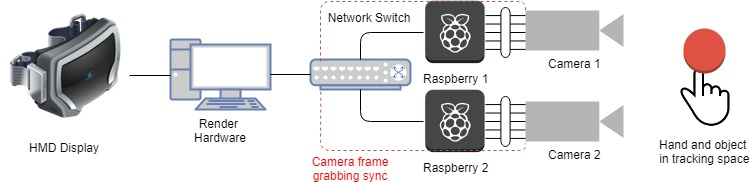
\includegraphics[width=\textwidth]{images/technical_setup.jpg}
\caption{Technical conseptiopn of the single hardware parts}
\label{technical-copnception}
\end{figure} 
The technical setup of the whole system is relatively simple. Instead of using one large dimmensioned Unit which takes care of all calculations, the image processing steps that have to be done on both stereo images anywy are outsourced onto the Raspberry Pis. As already mentioed in the conception Phase, the image processing dircetly on the rapspberry also reduces latency which would occur when sending image data over network channels to the main unit.\\
The two \textbf{Raspberry Pi 3 Model B}, which are used as the controllers for the\textbf{Raspberry Pi Camera V2} are connected via network cable to a network switch. A connection over wireless Network would be possible with the onboard capabilites of the  Pi's, but here we might encounter latency problems and/or signal interference with other exisitng networks. Therefor a cable connection is the safer solution.
The switch also connects to the "Master" PC to which the "Slave" Pi's communicate their data. The Master also takes care of the stereoscopic calculations,as it is dimensioned with far more computing power than the slaves.The 2D positional data from the slaves and dthe calculaton results from the stereo image disparity is fed into the hand Model running on the "Master". The model solutionis then applied to the digital hand model and rendered to the HMD.

 




